% Tex file for Ellen's PS4
% 8185: Quant Ellen PS2

\documentclass[12pt]{article}
%\usepackage[T1]{fontenc}
%\usepackage{lipsum}
\renewcommand{\baselinestretch}{1.2} 
\usepackage{graphicx}
\usepackage{hyperref}
\hypersetup{
    colorlinks=true,
    urlcolor=blue,
    citecolor=blue
}
\usepackage[export]{adjustbox}
\usepackage{subcaption}
\usepackage{comment}
\usepackage{amsmath}
\usepackage{amsfonts}
\usepackage{geometry}
\setcounter{MaxMatrixCols}{20}
\geometry{a4paper,
 left=3cm,right=3cm,
 top=1.5cm, bottom=1.5cm}

\usepackage{natbib}
\bibliographystyle{apalike}

%\usepackage{natbib}
%setcitestyle{authoryear,open={(},close={)}}
\graphicspath{ {../figs/} }

\begin{document}
%\thispagestyle{myheadings}
%\markright{Indian Statistical Institute, New Delhi\hfill }

\title{Econ 8185: Quant PS4}
\author{Bipul Verma}
\date{\today}
\maketitle

%\tableofcontents{}
\abstract{The present document use Finite Element Methods to calculate the policy functions.}

\vspace{8cm}

%\begin{center}
%\includegraphics[scale=0.4]{isi_logo.png}
%\end{center}
%\begin{center}
%\begin{Large}
%INDIAN STATISTICAL INSTITUTE, NEW-DELHI.
%\end{Large}
%\end{center}


\newpage

\section{Model}
Consider the simple neoclassical growth model with $\delta = 1$. 
\begin{align*}
\max_{c_t, k_{t+1}} \sum \beta^t log(c_t) \\
c_t + k_{t+1} = A k_t^{\alpha}
\end{align*}

The basic model has an analytical solution for the consumption policy function given by: $$c(k) = (1-\beta \alpha)Ak^{\alpha}.$$ We will approximate the policy function using finite elements methods as outlined below.

\subsection{Construction of Linear Basis}
We use the following formula to construct linear basis:
$$\psi_i(x) = 
\begin{cases}
\frac{x - x_{i-1}}{x_i - x{i-1}} & x \in [x_{i-1}, x_i] \\
\frac{x_{i+1} - x}{x_{i+1} - x_i} & x \in [x_i, x_{i+1}] \\
0 & \text{otherwise}
\end{cases}
$$
\textit{Note: The first and last basis is defined only on one of the relevant intervals.} We plot the basis for grid $X = [0,1, 3, 6]$ below: 
\begin{figure}[h]
\centering
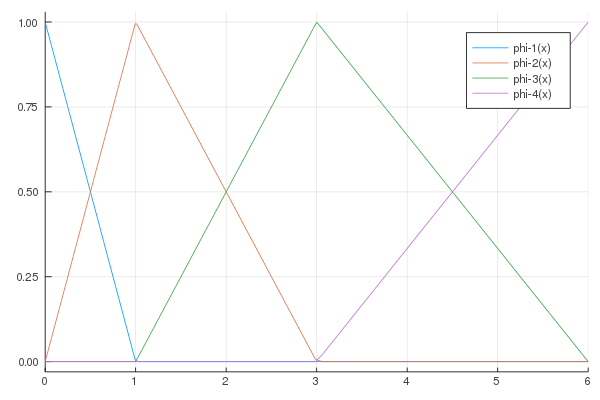
\includegraphics[scale=0.5]{linear_basisMM.png}
\caption{Piecewise Linear Basis Functions}
\end{figure}

\subsection{Estimation of Policy Function using Finite Elements}
We approximate the policy function as: $$c^n(k; \theta) = \sum_i \theta_i \psi_i(k).$$
The residual equation for the present case is: 
\begin{gather*}
R(k; \theta) = 1 - \beta \frac{c(k'; \theta)}{c(k; \theta)} A \theta (k')^{\alpha-1}\\
k' = Ak^\alpha - c(k; \theta)
\end{gather*}

We then use the Glarken Method to evaluate the integral of residual using weights same as the basis function. We set the weighted residual to zero: $$\int \psi_i(k)R(k; \theta)dk = 0.$$ For $i \in 1, 2, \dots n$, we have a system of equations. We stack the system and solve for $\theta$ using Newton Root finding method for vector valued functions. \textit{Note: We set $\theta_1=0$ to ensure $c^n(0; \theta) =0.$} Below is the estimated policy function plotted against the analytical policy function for different grid sizes.


\begin{figure}[h]
    \centering
    \begin{minipage}{0.45\textwidth}
        \centering
        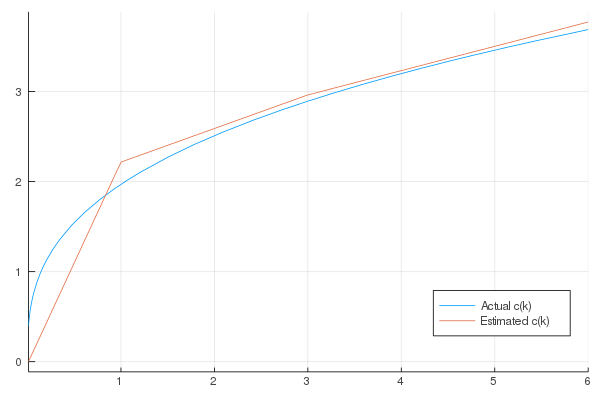
\includegraphics[width=1\textwidth]{c_policy_5grid.png} % first figure itself
        \caption{Estimated c(k) with 5 grid points}
    \end{minipage}\hfill
    \begin{minipage}{0.45\textwidth}
        \centering
        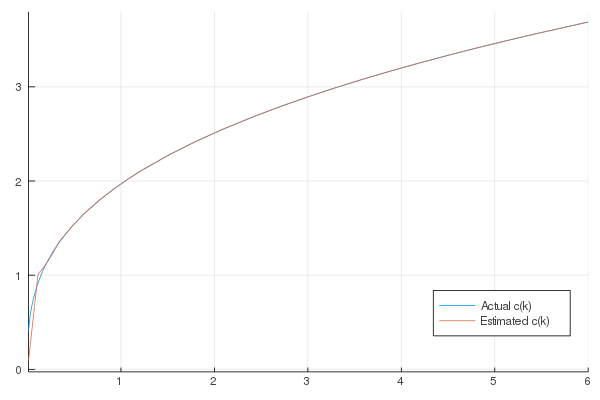
\includegraphics[width=1\textwidth]{c_policy_30grid.png} % second figure itself
        \caption{Estimated c(k) with 30 grid points}
    \end{minipage}
\end{figure}

We note that for decently sized grid, the estimated policy function is almost indistinguishable from the actual policy function for all points except near zero value of capital. To remedy this we can increase the number of grid points around zero. We'll use this idea in estimation of Aiyagari Model.

\newpage
\section{Application to basic Aiyagari Model}
The model is: 
\begin{gather*}
\max E_0 \sum \beta^t [c_t^{1-\mu} - 1]/(1-\mu) \\
\text{s.t. }\; \; c_t + a_{t+1} = w l_t + (1+r)a_t \\
c_t \geq 0, a_t \geq 0
\end{gather*}
where $l_t$ follows a finite state Markov process.

For the present case assume that $l_t$ is iid and takes two values $l_{L}$ and $l_{H}$ with equal probabilities. We can take into account the non-negativity constraint by taking into adding a penalty  as outlined in the notes. The final Residual equation obtained for this model is:
\begin{gather*}
R(a, l_t) = \beta(1+r) E[c'^{-\mu}] + \beta \zeta \min(a', 0)^2 - c^{-\mu}\\
c(a) = wl_t + (1+r)a - a'(a, l_t)\\
E[c'(a'(a, l_t), l_{t+1})^{-\mu}] = E_{l_{t+1}}[(wl_{t+1} +(1+r)a'(a, l_t) - a'(a'(a, l_t), l_{t+1}))^{-\mu}]
\end{gather*}

Since there are two states for $l_t$, we'll have a asset policy function corresponding to $l_L$ and $l_H$. We approximate the polcy function as follows:
\begin{gather*}
a'^n(a; \theta^L) = \sum_i \psi_i(a)\theta^L_i \\
a'^n(a; \theta^H) = \sum_i \psi_i(a)\theta^H_i \\
\theta = [\theta^L, \theta^H]'
\end{gather*}

As outlined in the previous section we solve a system of equations by setting weighted residuals to zero, where the weights are same as the basis function. 

\subsection{Results}
For the present case we use the following parameter specification (taken from Fran's PS):
\begin{align*}
\beta = 0.9 \\
\mu = 2 \\
w = 1.17 \\
r = 0.04 \\
\zeta = 30000 \\
l_L = 0.4, l_H = 1
\end{align*}

We build the asset grid to be between 0 and 20, with 20 exponentially increasing points. We make sure to add more points near zero to account for asset constraint binding. Below we plot the estimated asset policy function for the two states of labor.\\
\newpage

\begin{figure}[h]
    \centering
    \begin{minipage}{0.45\textwidth}
        \centering
        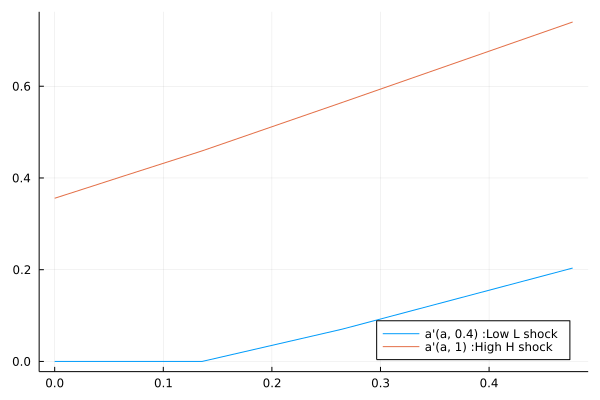
\includegraphics[width=1\textwidth]{a_policy_aiyagari.png} % first figure itself
        \caption{Asset Policy function near zero assets}
    \end{minipage}\hfill
    \begin{minipage}{0.45\textwidth}
        \centering
        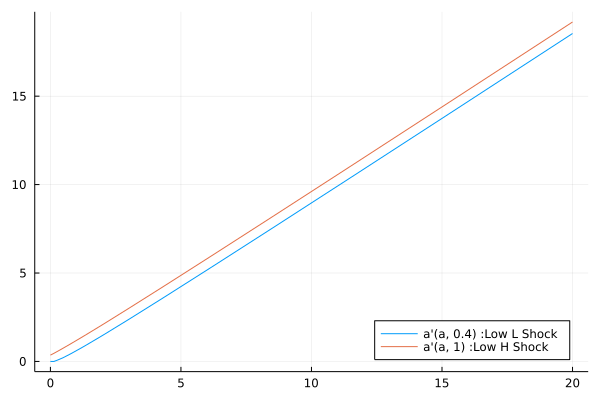
\includegraphics[width=1\textwidth]{a_policy_aiyagari_new.png} % second figure itself
        \caption{Asset policy function}
    \end{minipage}
\end{figure}


\begin{comment}
\begin{figure}[htp]
\centering
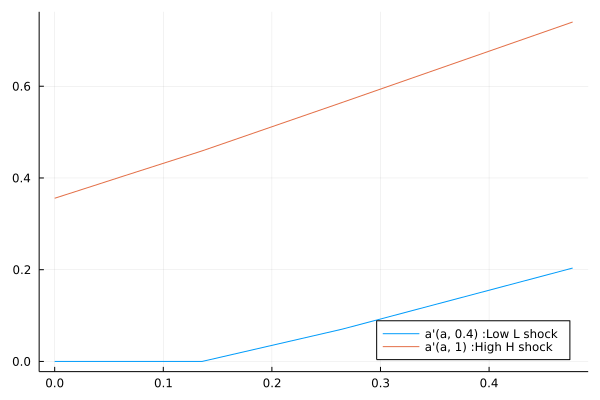
\includegraphics[scale=0.5]{a_policy_aiyagari.png}
\caption{Basic Aiyagari asset policy function}
\end{figure}
\end{comment}

\subsubsection{Discussion of Results}
We note that the asset constraint is binding for the low productivity agent ($l = 0.4$) at very low level of asset. At high level of assets the asset constraint is no longer binding and the curve is upward sloping. For the high productivity agent ($l = 1$), the asset policy function is upward sloping at all assets with a positive intercept. 

%\newpage
%\bibliography{ref}

\end{document}